\documentclass{article}
\usepackage{graphicx} % Required for inserting images
\usepackage{fancyhdr} % Header
\usepackage{lastpage}
\usepackage[a4paper, total={6in, 8in}]{geometry}
\usepackage{float} % Floating position
\usepackage{hyperref} % Links
\usepackage{amsmath} % Math
\usepackage{amssymb} % Math
\usepackage{bbold} % Math (for indicatrice function)
\usepackage{listings} % Import code in appendix
\usepackage{xcolor} % For coloring code
% Listing Configuration
\lstset{
    language=Python,
    basicstyle=\ttfamily\small,
    keywordstyle=\color{blue},
    stringstyle=\color{red},
    commentstyle=\color{green},
    showstringspaces=false,
    breaklines=true,
    frame=single
}
\usepackage{tikz} % Graph
\usetikzlibrary{bayesnet}
\usetikzlibrary{positioning}

\graphicspath{{images/}}

\newcommand{\authorFst}{Tristan Perrot}
\newcommand{\emailFst}{\href{mailto:tristanp@kth.se}{tristanp@kth.se}}

\pagestyle{fancy}
\fancyhf{} % clear all header and footer fields
\lhead{Assignment 1B \\ DD2434 - Machine Learning, Advanced Course}
\rhead{\authorFst}
\cfoot{\thepage \  / \pageref{LastPage}}
\setlength{\headheight}{23pt}
\setlength{\footskip}{70pt}

\title{DD2434 - Machine Learning, Advanced Course \\ Assignment 1B}
\author{\authorFst \\ \emailFst}
\date{November 2023}

\begin{document}

\maketitle

\begin{center}
  
\includegraphics[scale=0.5]{KTH_logo_RGB_bla.png}
\end{center}

\thispagestyle{empty}

\newpage
\tableofcontents
\newpage

\section{CAVI for Earth quakes}

\subsection{Question 1.1}

\begin{figure}[H]
  \centering
  \begin{tikzpicture}

  % Define nodes
  \node[latent] (theta) {$\theta_d$};
  \node[latent, left=of theta] (alpha) {$\alpha$};
  \node[latent, right=of theta] (z) {$Z_{d,n}$};
  \node[latent, right=of z] (w) {$W_{d,n}$};
  \node[latent, right=of w] (beta) {$\beta_k$};
  \node[latent, right=of beta] (eta) {$\eta$};

  % Connect nodes
  \edge {alpha} {theta}
  \edge {theta} {z}
  \edge {z} {w}
  \edge {beta} {w}
  \edge {eta} {beta}

  % Plates
  \plate [inner xsep=0.3cm] {plate1} {(z)(w)} {$N$}
  \plate [inner xsep=0.3cm] {plate2} {(theta)(z)(w)(plate1)} {$D$}
  \plate [inner xsep=0.2cm, xshift=0.1cm] {plate3} {(beta)} {$K$}

\end{tikzpicture}

  \label{fig:fig1}
  \caption{Directed Graphical Model for the Earthquake problem}
\end{figure}

\subsection{Question 1.2}

Here, we know these distributions:
\begin{itemize}
  \item $p(Z_n|\pi) = Categorical(\pi)$
  \item $p(S_n|Z_n = k, \lambda_k) = Poisson(\lambda_k)$
  \item $p(X_n|Z_n = k, \mu_k, \tau) = Normal(\mu_k, \tau \cdot I)$
  \item $p(\mu_k|\nu,\rho) = Normal(\nu, \rho \cdot I)$
  \item $p(\lambda_k|\alpha, \beta) = Gamma(\alpha, \beta)$
\end{itemize}
Where, $\rho$ and $\tau$ define precision and not standard variation. Then we have:
\begin{equation}
  \begin{split}
    \log p(X,S,Z,\lambda,\mu|\pi,\tau,\alpha,\beta,\nu,\rho) & = \log p(X|S,Z,\lambda,\mu,\pi,\tau,\alpha,\beta,\nu,\rho)                 \\
                                                             & \qquad\qquad + \log p(S,Z,\lambda,\mu|\pi,\alpha,\beta,\nu,\rho)           \\
                                                             & = \log p(X|Z,\mu,\tau) + \log p(S|Z,\lambda,\mu,\pi,\alpha,\beta,\nu,\rho) \\
                                                             & \qquad\qquad + \log p(Z,\lambda,\mu|\pi\alpha,\beta,\nu,\rho)              \\
                                                             & = \log p(X|Z,\mu,\tau) + \log p(S|Z,\lambda) + \log p(Z|\pi)               \\
                                                             & \qquad\qquad + \log p(\lambda,\mu|\alpha,\beta,\nu,\rho)                   \\
    \log p(X,S,Z,\lambda,\mu|\pi,\tau,\alpha,\beta,\nu,\rho) & = \log p(X|Z,\mu,\tau) + \log p(S|Z,\lambda) + \log p(Z|\pi)               \\
                                                             & \qquad\qquad + \log p(\mu|\nu,\rho) + \log p(\lambda|\alpha,\beta)         \\
  \end{split}
\end{equation}

Where:
\begin{equation}
  \begin{split}
    \log p(X|Z,\mu,\tau)         & = \sum_{n=1}^{N}\sum_{k=1}^{K}\log p(X_n|Z_n = k, \mu_k, \tau) \\
    \log p(S|Z,\lambda)          & = \sum_{n=1}^{N}\sum_{k=1}^{K}\log p(S_n|Z_n = k, \lambda_k)   \\
    \log p(Z|\pi)                & = \sum_{n=1}^{N}\log p(Z_n|\pi)                                \\
    \log p(\mu|\nu,\rho)         & = \sum_{k=1}^{K}\log p(\mu_k|\nu,\rho)                         \\
    \log p(\lambda|\alpha,\beta) & = \sum_{k=1}^{K}\log p(\lambda_k|\alpha,\beta)                 \\
  \end{split}
\end{equation}

\subsection{Question 1.3}

Here, the mean field approximation is not an approximation but an equality because $Z, \mu, \lambda$ are independent. Therefore we have:
\begin{equation}
  \begin{split}
    \log q^*(Z_n) & \overset{+}{=} \mathbb{E}_{\mu,\lambda}[\log p(X_n,S_n,Z_n,\lambda,\mu|\pi,\tau,\alpha,\beta,\nu,\rho)]                                                                                                               \\
                  & \overset{+}{=} \mathbb{E}_{\mu,\lambda}[\log p(X_n|Z_n,\mu,\tau) + \log p(S_n|Z_n,\lambda) + \log p(Z_n|\pi)]                                                                                                         \\
                  & = \mathbb{E}_{\mu}\left[\sum_{k=1}^{K}\mathbb{1}_{\{Z_n = k\}}\left(\log \left(\frac{\tau}{2\pi}\right) -\frac{\tau}{2}\left((x_n - \mu_k)^T(x_n - \mu_k)\right)\right)\right]                                        \\
                  & \qquad\qquad + \mathbb{E}_{\lambda}\left[\sum_{k=1}^{K}\mathbb{1}_{\{Z_n = k\}}\left(\log(\pi_k) + \sum_{j \in \mathbb{N}}\mathbb{1}_{\{S_n = j\}}\left[-\lambda_k + j\log(\lambda_k) - \log(j!)\right]\right)\right] \\
                  & \overset{+}{=} \sum_{k=1}^{K}\mathbb{1}_{\{Z_n = k\}}\left(\log \left(\frac{\tau}{2\pi}\right) - \frac{\tau}{2}\mathbb{E}_{\mu}\left[(x_n - \mu_k)^T(x_n - \mu_k)\right] \right.                                      \\
                  & \qquad\qquad \left. + \log(\pi_k) + \sum_{j \in \mathbb{N}}\mathbb{1}_{\{S_n = j\}}\mathbb{E}_{\lambda}\left[-\lambda_k + j\log(\lambda_k) - \log(j!)\right]\right)
  \end{split}
\end{equation}
Now, if we take the entire expression that is multiplied by $\mathbb{1}_{\{Z_n = k\}}$ and we call it $u_{n,k}$, we have:
\begin{equation}
  q^*(Z_n) \overset{+}{=} \prod_{k=1}^{K}u_{n,k}^{\mathbb{1}_{\{Z_n = k\}}}
\end{equation}
And if we normalize by taking $r_{n,k} = \frac{u_{n,k}}{\sum_{i=1}^{K}u_{n,i}}$ we get:
\begin{equation}
  q^*(Z_n) \overset{+}{=} \prod_{k=1}^{K}r_{n,k}^{\mathbb{1}_{\{Z_n = k\}}}
\end{equation}
Wich means that $q^*(Z_n)$ is a categorical distribution with parameters $r_{n,k}$. There for we have the expectation of $Z_n$ easily because $\mathbb{E}[z_{n,k}] = r_{n,k}$ where $z_{n,k} = \mathbb{1}_{\{S_n = k\}}$. Note that $r_{n,k}$ depends of the expected value of $\mu_k$, $\mu_k^2$, $\lambda_k$ and $\log \lambda_k$. We will be able to compute these expected values by finding $q^*(\mu_k)$ and $q^*(\lambda_k)$.

\noindent Let us compute $q^*(\mu_k)$:
\begin{equation}
  \begin{split}
    \log q^*(\mu_k) & \overset{+}{=} \mathbb{E}_{Z,\lambda}[\log p(X,S,Z = k,\lambda_k,\mu_k|\pi,\tau,\alpha,\beta,\nu,\rho)]                                                                                                  \\
                    & \overset{+}{=} \mathbb{E}_{Z,\lambda}[\log p(X|Z = k,\mu_k,\tau) + \log p(\mu_k|\nu,\rho)]                                                                                                               \\
                    & = \mathbb{E}_{Z,\lambda}\left[\sum_{n=1}^{N}\mathbb{1}_{\{Z_n = k\}}\left(\log \left(\frac{\tau}{2\pi}\right) -\frac{\tau}{2}\left((x_n - \mu_k)^T(x_n - \mu_k)\right)\right)\right]                     \\
                    & \qquad\qquad + \log \left(\frac{\rho}{2\pi}\right) - \frac{\rho}{2}\left((\mu_k - \nu)^T(\mu_k - \nu)\right)                                                                                             \\
                    & \overset{+}{=} \sum_{n=1}^{N}r_{n,k}\left(\log \left(\frac{\tau}{2\pi}\right) - \frac{\tau}{2}\left((x_n - \mu_k)^T(x_n - \mu_k)\right)\right) - \frac{\rho}{2}\left((\mu_k - \nu)^T(\mu_k - \nu)\right) \\
  \end{split}
\end{equation}

\newpage
\appendix

\section{Appendix}
\subsection{Question 1.2}\label{appendix:code.1.2}
\lstinputlisting[label = {alg:3.12}]{py_files/1.2.py}

\end{document}